\chapter{Impact of Oppression}
\begin{figure}[h]
\centering
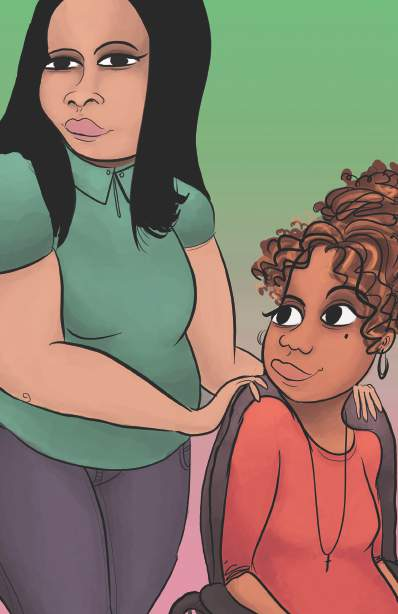
\includegraphics[height=12cm]{TeX_files/2-0.png}
\caption{Artist: Mohammed Fayaz}
\label{2-0}
\end{figure}


\newpage
\begin{figure}[h]
\centering
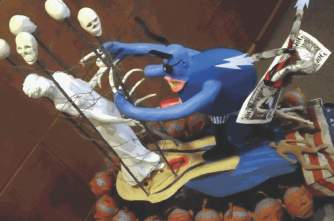
\includegraphics[width=16cm]{TeX_files/2-1.png}
\caption{Artist: JW Arndt}
\label{2-1}
\end{figure}

\noindent\textcolor{ProcessBlue}{\textbf{\Large{How does oppression affect your feelings?}}}\\
\large{\textbf{Here are some emotions we identified:}}
\begin{multicols}{3}
\begin{itemize}
\item[$\square$]{Angry}
\item[$\square$]{Restless}
\item[$\square$]{Emotionally fatigued}
\item[$\square$]{Enraged}
\item[$\square$]{Sad}
\item[$\square$]{Despaired}
\item[$\square$]{Sorrowed}
\item[$\square$]{Helpless}
\item[$\square$]{Powerless}
\item[$\square$]{Ashamed}
\item[$\square$]{Worried}
\item[$\square$]{Embarassed}
\item[$\square$]{Frustrated}
\item[$\square$]{Worthless}
\item[$\square$]{Anxious}
\item[$\square$]{Betrayed}
\item[$\square$]{Confused}
\item[$\square$]{Isolated}
\item[$\square$]{Physically Fatigued}
\item[$\square$]{Rebellious}
\item[$\square$]{Empty}
\item[$\square$]{Humiliated}
\item[$\square$]{Distrustful}
\item[$\square$]{Upset}
\item[$\square$]{Despondent}
\item[$\square$]{Disorientated}
\item[$\square$]{Defensive}
\item[$\square$]{Indignant}
\item[$\square$]{Impatient}
\item[$\square$]{Hostile}
\item[$\square$]{Tense}
\item[$\square$]{Hurt}
\item[$\square$]{Disillusioned}
\item[$\square$]{Alienated}
\end{itemize}
\end{multicols}


\newpage
\noindent
\textcolor{ProcessBlue}{\textbf{\Large{What other emotions do you feel when you experience oppression?}}}\\\\
\noindent\rule{\textwidth}{1pt}\\
\noindent\rule{\textwidth}{1pt}\\
\noindent\rule{\textwidth}{1pt}\\
\noindent\rule{\textwidth}{1pt}\\
\noindent\rule{\textwidth}{1pt}\\
\noindent\rule{\textwidth}{1pt}\\
\noindent\rule{\textwidth}{1pt}\\
\noindent\rule{\textwidth}{1pt}\\\\

\noindent\textcolor{ProcessBlue}{\textbf{\Large{How does oppression affect your behavior?}}}\\
\textbf{\large{Here are some ways we described:}}
\begin{multicols}{2}
\begin{itemize}
\item[$\square$]{I hide.}
\item[$\square$]{I overeat.}
\item[$\square$]{I am unable to eat}
\item[$\square$]{I oversleep}
\item[$\square$]{I get insomnia}
\item[$\square$]{I lash out}
\item[$\square$]{I need physical distance from people}
\item[$\square$]{I act crazy}
\item[$\square$]{I become submissive}
\item[$\square$]{I get violent}
\item[$\square$]{I freeze}
\item[$\square$]{I stop talking}
\item[$\square$]{I stutter}
\item[$\square$]{I collapse emotionally}
\item[$\square$]{I stop taking care of myself}
\item[$\square$]{I have nightmares}
\item[$\square$]{I become passive aggressive}
\item[$\square$]{I look for payback}
\item[$\square$]{I become fearful of the future}
\item[$\square$]{I feel my life is about to fall apart}
\item[$\square$]{I disassociate}
\item[$\square$]{I withdraw}
\item[$\square$]{I retreat}
\item[$\square$]{I escape into an imaginary world}
\item[$\square$]{I convulse}
\item[$\square$]{I freeze}
\end{itemize}
\end{multicols}


\newpage
\noindent
\textcolor{ProcessBlue}{\textbf{\Large{How does oppression affect the way you behave?}}}\\\\
\noindent\rule{\textwidth}{1pt}\\
\noindent\rule{\textwidth}{1pt}\\
\noindent\rule{\textwidth}{1pt}\\
\noindent\rule{\textwidth}{1pt}\\
\noindent\rule{\textwidth}{1pt}\\
\noindent\rule{\textwidth}{1pt}\\
\noindent\rule{\textwidth}{1pt}\\
\noindent\rule{\textwidth}{1pt}\\\\

\noindent\textcolor{ProcessBlue}{\textbf{\Large{How does oppresion make you sick?}}}\\
\textbf{\large{Here are some ways we identified:}}
\begin{multicols}{2}
\begin{itemize}
\item[$\square$]{I have tried to commit suicide}
\item[$\square$]{I have suicidal thoughts}
\item[$\square$]{I have panic attacks}
\item[$\square$]{I get headaches}
\item[$\square$]{I get stomach aches}
\item[$\square$]{I experience depression}
\item[$\square$]{I feel anxiety and paranoia}
\item[$\square$]{I get persistent negative thoughts}
\item[$\square$]{I feel dizziness}
\item[$\square$]{I have developed eating disorders}
\item[$\square$]{I abuse alcohol and/or drugs}
\item[$\square$]{I have nightmares}
\item[$\square$]{I experience sleep disturbance}
\item[$\square$]{I have developed an ulcer}
\item[$\square$]{All of my symptoms escalate}
\item[$\square$]{Fear and paranoia of healthcare}
\item[$\square$]{I self harm}
\item[$\square$]{Self-hate}
\item[$\square$]{I have insomnia}
\item[$\square$]{It triggers manic episodes}
\item[$\square$]{I experience PTSD}
\item[$\square$]{I become ''delusional''}
\item[$\square$]{I become ''psychotic''}
\item[$\square$]{I dissociate}
\item[$\square$]{I get rashes}
\item[$\square$]{I develop compulsive behavior}
\item[$\square$]{I exhibit obsessive behavior}
\item[$\square$]{I get depressed}
\end{itemize}
\end{multicols}


\newpage
\noindent
\textcolor{ProcessBlue}{\textbf{\Large{How does oppression manifest in your body and mind?}}}\\\\
\noindent\rule{\textwidth}{1pt}\\
\noindent\rule{\textwidth}{1pt}\\
\noindent\rule{\textwidth}{1pt}\\
\noindent\rule{\textwidth}{1pt}\\
\noindent\rule{\textwidth}{1pt}\\
\noindent\rule{\textwidth}{1pt}\\
\noindent\rule{\textwidth}{1pt}\\
\noindent\rule{\textwidth}{1pt}\\\\

\noindent\textcolor{ProcessBlue}{\textbf{\Large{How do microaggressions compromise your wellness?}}}\\
\textbf{\large{Here is how some of us described the experience:}}
\begin{multicols}{2}
\begin{itemize}
\item[$\square$]{Self-shame}
\item[$\square$]{Racing pulse}
\item[$\square$]{I get really upset or agitated}
\item[$\square$]{I exhibit excessive aggression}
\item[$\square$]{I get violent}
\item[$\square$]{I self-harm}
\item[$\square$]{I get scared}
\item[$\square$]{I get frustrated.}
\item[$\square$]{I feel sad and memories come back in waves.}
\item[$\square$]{I get distracted and lose focus}
\item[$\square$]{I underperform}
\item[$\square$]{I feel anxiety}
\item[$\square$]{Intrusive thoughts}
\item[$\square$]{Ear ringing}
\item[$\square$]{Heat waves}
\item[$\square$]{Flashbacks}
\item[$\square$]{Agitation}
\item[$\square$]{Fear}
\item[$\square$]{Sadness}
\item[$\square$]{Anxiety}
\item[$\square$]{Hypervigilance}
\item[$\square$]{Quickening of the pulse}
\item[$\square$]{Anger}
\item[$\square$]{Disorientation}
\item[$\square$]{Dizziness}
\item[$\square$]{Nausea}
\item[$\square$]{Shakiness}
\end{itemize}
\end{multicols}


\newpage
\noindent
\textcolor{ProcessBlue}{\textbf{\Large{In what other ways do microaggressions compromise your wellness?}}}\\
\noindent\rule{\textwidth}{1pt}\\
\noindent\rule{\textwidth}{1pt}\\
\noindent\rule{\textwidth}{1pt}\\
\noindent\rule{\textwidth}{1pt}\\
\noindent\rule{\textwidth}{1pt}\\
\noindent\rule{\textwidth}{1pt}\\
\noindent\rule{\textwidth}{1pt}\\
\noindent\rule{\textwidth}{1pt}\\
\noindent\rule{\textwidth}{1pt}\\\\

\noindent\textcolor{ProcessBlue}{\textbf{\Large{How does oppression affect the way you see yourself?}}}\\
\textbf{\large{Here are some ways we identified:}}
\begin{multicols}{2}
\begin{itemize}
\item[$\square$]{I feel really bad about myself}
\item[$\square$]{I feel like I would rather just not be around}
\item[$\square$]{I become egocentric}
\item[$\square$]{I get angry with myself}
\item[$\square$]{I have self-loathing}
\item[$\square$]{I get caught in trying to fit an ideal of myself, rather than honestly being myself}
\item[$\square$]{I question my ability to achieve goals}
\item[$\square$]{I question if I will ever have happiness}
\item[$\square$]{I am concerned that I am not “worthy” of being loved}
\item[$\square$]{I feel so undermined}
\item[$\square$]{I wonder if I’m just doing it all wrong, which quickly leads to feeling worse}
\item[$\square$]{I feel distant from myself, fractured and uncertain about the future}
\item[$\square$]{I feel unfocused and disengaged}
\item[$\square$]{I blame myself}
\item[$\square$]{I think, “Shouldn’t have done that!”}
\item[$\square$]{It makes it hard to feel strong and effective in the world}
\item[$\square$]{Every time it happens, I have to restart the relationship with myself}
\item[$\square$]{The shame and hate stay with me, it’s very difficult to move past them}
\item[$\square$]{The shame and hate stay with me, it’s very difficult to move past}
\item[$\square$]{I observe my mind whirling with anger, guilt, frustration}
\item[$\square$]{I doubt myself}
\item[$\square$]{I have decreased confidence in my ability to interact with others and to judge others}
\item[$\square$]{I feel desperate and worthless going over old hurts}
\item[$\square$]{I cannot cope with the idea of future hurts}
\item[$\square$]{I have switching and ‘shifts’ that can look like mood swings from the outside, but aren’t}
\item[$\square$]{I often struggle with self hatred and shame}
\item[$\square$]{I fee “less than” and inferior to my peers}
\item[$\square$]{I often feel alienated from myself}
\end{itemize}
\end{multicols}

\begin{figure}[h]
\centering
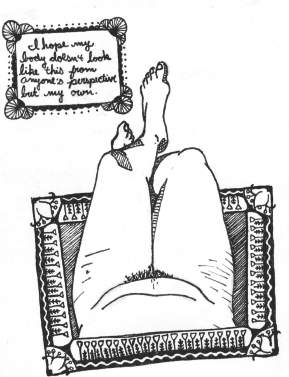
\includegraphics[height=16cm]{TeX_files/2-2.png}
\caption{Artist: Jodi Bentivegna}
\label{2-2}
\end{figure}

\newpage
\noindent
\textcolor{ProcessBlue}{\textbf{\Large{How does oppression affect the way you perceive yourself?}}}\\
\noindent\rule{\textwidth}{1pt}\\
\noindent\rule{\textwidth}{1pt}\\
\noindent\rule{\textwidth}{1pt}\\
\noindent\rule{\textwidth}{1pt}\\
\noindent\rule{\textwidth}{1pt}\\
\noindent\rule{\textwidth}{1pt}\\
\noindent\rule{\textwidth}{1pt}\\
\noindent\rule{\textwidth}{1pt}\\\\

\noindent\textcolor{ProcessBlue}{\textbf{\Large{What are the social consequences of oppression?}}}\\
\textbf{\large{It affects our relationships with friends, family, and partners in these ways:}}
\begin{multicols}{2}
\begin{itemize}
\item[$\square$]{I have no friends}
\item[$\square$]{My family doesn’t talk to me}
\item[$\square$]{I isolate myself}
\item[$\square$]{I lash out in anger at my family and friends}
\item[$\square$]{After I began to speak out, my family began treating me as a villain and telling me I am selfish}
\item[$\square$]{Friends who don’t understand oppression do not fully know me because they don’t have that context}
\item[$\square$]{I have to struggle with my internal conditioned reactions to sex that signal “danger, you’re being used” so that I can experience it differently (meaning positively) or even experience it at all and not be checked out}
\item[$\square$]{I feel resentful}
\item[$\square$]{It makes me cautious}
\item[$\square$]{I have difficulty trusting myself or others}
\item[$\square$]{It makes communication very challenging}
\item[$\square$]{It makes it difficult for me to be comfortable in group situations}
\item[$\square$]{I have difficulty socializing with and expressing affection safely with others}
\item[$\square$]{Sometimes act like I am being oppressed in relationships even when I am not}
\end{itemize}
\end{multicols}


\newpage
\textbf{\large{It affects our broader community in these ways:}}
\begin{multicols}{2}
\begin{itemize}
\item[$\square$]{I isolate}
\item[$\square$]{I’m alienated from all but my peers}
\item[$\square$]{I still have a hard time believing I will be accepted and trusted by people }
\item[$\square$]{My circles are somewhat small and I don’t have relationships from when I was younger }
\item[$\square$]{Sometimes I realize it takes me a long time to accomplish what other folks might see as simple communications}
\item[$\square$]{I limit how much I connect with people around me in public places and in the community because of my lack of confidence and fear of not being accepted or respected}
\item[$\square$]{Feeling that I cannot expect to feel safe in the broader world leads me to being timid and half present}
\item[$\square$]{I don’t feel a sense of belonging to my broader community}
\item[$\square$]{My interactions are limited and superficial. I put on a happy face and stay in line}
\item[$\square$]{I can’t let anyone know my struggles}
\item[$\square$]{I am utterly convinced that the wider community despises me and wants nothing to do with me}
\item[$\square$]{I feel I have nothing to offer, or give, or do}
\item[$\square$]{It makes it difficult to find a place and a way to contribute meaningfully to the community}
\end{itemize}
\end{multicols}

\noindent
\textcolor{ProcessBlue}{\textbf{\Large{What other social consequences of oppression do you experience?}}}\\
\noindent\rule{\textwidth}{1pt}\\
\noindent\rule{\textwidth}{1pt}\\
\noindent\rule{\textwidth}{1pt}\\
\noindent\rule{\textwidth}{1pt}\\
\noindent\rule{\textwidth}{1pt}\\
\noindent\rule{\textwidth}{1pt}\\
\noindent\rule{\textwidth}{1pt}\\
\noindent\rule{\textwidth}{1pt}\\
\noindent\rule{\textwidth}{1pt}\\\\


\newpage
\begin{figure}[h]
\centering
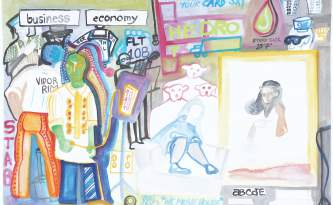
\includegraphics[width=16cm]{TeX_files/2-3.png}
\caption{Artist: Eddy Falconer}
\label{2-2}
\end{figure}

\noindent\textcolor{ProcessBlue}{\textbf{\Large{How does oppression affect your ability to work?}}}\\
\textbf{\large{Here are some ways we identified:}}
\begin{multicols}{2}
\begin{itemize}
\item[$\square$]{I can’t work when I am sleeping 24/7}
\item[$\square$]{The medications make it harder for me to appear natural when interacting with coworkers or classmates}
\item[$\square$]{I quit my jobs constantly, because there are behaviors that trigger my depressive periods and I can’t do my job well}
\item[$\square$]{I’ve had 42 jobs. It is damn near impossible for me to keep one. While highly skilled and resilient with a strong network, I can’t keep myself in work for very long}
\item[$\square$]{To be honest, I don’t even know how I can really work...but of course I can’t not, so it’s just a perpetual painful mess}
\item[$\square$]{Going to work is the hardest part}
\item[$\square$]{Trying to interact with people who don’t understand and don’t want to makes me feel like giving up, so I keep to myself a lot and try my best to find jobs that don’t require others}
\item[$\square$]{I can’t work anymore. I suspect that’s a reaction to the oppression}
\item[$\square$]{I have often debilitating anxiety related to PTSD, and it has kept me in very part time jobs, as I am worried to take on too much responsibility}
\item[$\square$]{I am worried about having attacks and not feeling able to explain why I can’t work}
\end{itemize}
\end{multicols}


\newpage
\noindent
\textcolor{ProcessBlue}{\textbf{\Large{How does oppression affect your daily life and your ability to work?}}}\\
\noindent\rule{\textwidth}{1pt}\\
\noindent\rule{\textwidth}{1pt}\\
\noindent\rule{\textwidth}{1pt}\\
\noindent\rule{\textwidth}{1pt}\\
\noindent\rule{\textwidth}{1pt}\\
\noindent\rule{\textwidth}{1pt}\\
\noindent\rule{\textwidth}{1pt}\\
\noindent\rule{\textwidth}{1pt}\\
\noindent\rule{\textwidth}{1pt}\\\\

\noindent\textcolor{ProcessBlue}{\textbf{\Large{What are the social consequences of oppression?}}}\\
\textbf{\large{It affects our relationships with friends, family, and partners in these ways:}}
\begin{multicols}{2}
\begin{itemize}
\item[$\square$]{It makes my life marginal, disorganized, and pathetic}
\item[$\square$]{Fighting against overeating and other self-destructive habits has taken a lot of my time}
\item[$\square$]{Mental illness is invisible}
\item[$\square$]{Daily life hurts like hell}
\item[$\square$]{Fifteen years of antipsychotics have taken their toll}
\item[$\square$]{Constant pain}
\item[$\square$]{Constantly containing my overflowing container}
\item[$\square$]{Constant worry and feelings of being “lost”}
\item[$\square$]{I wake up depressed...everyday is the same and there is nothing to do and no one to talk to}
\item[$\square$]{I am always looking for police. I don’t fear people in my neighborhood, I just fear police when I see them}
\item[$\square$]{I put off things like cleaning or doing the dishes and lose myself online}
\item[$\square$]{My daily life is a moment to moment challenge to experience my own perspective, be comfortable in my own skin, to find meaning and connection and a reason to continue living}
\item[$\square$]{There are days when just having to get out of bed makes me want to cry}
\item[$\square$]{Having to leave the house almost always breaks my heart}
\item[$\square$]{Being responsible is difficult. It’s hard to take care of myself}
\end{itemize}
\end{multicols}


\newpage
\noindent
\noindent\rule{\textwidth}{1pt}\\
\noindent\rule{\textwidth}{1pt}\\
\noindent\rule{\textwidth}{1pt}\\
\noindent\rule{\textwidth}{1pt}\\
\noindent\rule{\textwidth}{1pt}\\
\noindent\rule{\textwidth}{1pt}\\
\noindent\rule{\textwidth}{1pt}\\
\noindent\rule{\textwidth}{1pt}\\
\noindent\rule{\textwidth}{1pt}\\
\noindent\rule{\textwidth}{1pt}\\
\noindent\rule{\textwidth}{1pt}\\
\noindent\rule{\textwidth}{1pt}\\
\noindent\rule{\textwidth}{1pt}\\
\noindent\rule{\textwidth}{1pt}\\
\noindent\rule{\textwidth}{1pt}\\
\noindent\rule{\textwidth}{1pt}\\
\noindent\rule{\textwidth}{1pt}\\
\noindent\rule{\textwidth}{1pt}\\
\noindent\rule{\textwidth}{1pt}\\
\noindent\rule{\textwidth}{1pt}\\
\noindent\rule{\textwidth}{1pt}\\
\noindent\rule{\textwidth}{1pt}\\
\noindent\rule{\textwidth}{1pt}\\
\noindent\rule{\textwidth}{1pt}\\
\noindent\rule{\textwidth}{1pt}\\
\noindent\rule{\textwidth}{1pt}\\
\noindent\rule{\textwidth}{1pt}\\
\noindent\rule{\textwidth}{1pt}\\


